\scanpage{8}
Supposons que $q\alpha-\alpha'\ne0$ alors
\[
\begin{aligned}
(1)\ \Longrightarrow\quad &p\mid\sum_{i=1}^{q-1}C_q^i\,a^i b'^{\,q-i-1}+b'^{\,q-1}\\
\Longrightarrow\quad &p\mid q\,a^{q-1}\qquad\text{car }p\mid b'\ \text{et pour }i\ne q-1\quad q-i-1\deleted{\ne0}>0
\end{aligned}
\]
or $p\mid b'$ et $b'\mid b^q$ donc $b'\mathrel{\underset{1}{\smile}}a$ donc $p\mathrel{\underset{1}{\smile}}a$

\deleted{donc si $\unsure{p\ne1|p\ne q}$}
\[
(1)\ \Longrightarrow\quad p\mid q\qquad\text{donc }\deleted{p=1\ \text{ou }}p=q\quad(\text{si }q\alpha-\alpha'\ne0)
\]
Donc si $p\ne q$ \quad $p$ premier \inserted{ou $p=1$} et $p\mid b'$ alors $\alpha'=q\alpha$ \deleted{(on l'impose sans risque si $p=1$)}

Donc $\exists\,b_0\in\mathbb N^*$ et $\exists\,\gamma\in\mathbb N$ tel que $b'=q^\gamma b_0^q$ \margin{$q\nmid b_0$}

de plus $b_0\mid b$ et si $b=b_0 b''$ alors $b_0\mathrel{\underset{1}{\smile}}b''$ ?

De même $\exists\,a_0\in\mathbb N^*$ et $\exists\,\unsure{\zeta|\delta}\in\mathbb N$ tel que $a'=q^\zeta a_0^q$ avec $a_0\mid a$ et si $a=a_0a''$ alors $a_0\mathrel{\underset{1}{\smile}}a''$ ?

or $a\mathrel{\underset{1}{\smile}}b\Longrightarrow a_{\deleted{\unsure{0}}}'\mathrel{\underset{1}{\smile}}b'\Longrightarrow\zeta\times\gamma=0$ (et aussi $a_0\mathrel{\underset{1}{\smile}}b_0$)

Je suppose désormais que $\zeta=0$ donc $a'=a_0^q$

Donc \quad $c=b+a_0^q=a+q^\gamma b_0^q$
\margin{\begin{tikzpicture}[baseline=(n.base)]
\node[inner sep=2pt,text width=.85\marginparwidth] (n) {pour $q=2$ on a, $a_0=b_0=1$, $\gamma=1$, $b=4$, $a=3$, $c=5$};
\draw (n.north east) -- (n.north west) -- (n.south west) -- (n.south east);
\end{tikzpicture}}

\noindent\rule{\linewidth}{.35pt}\par
Je fais l'hypothése suivante \quad si $q$ premier et $1\leqslant i<q$ alors $q\mid C_q^i$
\par\noindent\rule{\linewidth}{.35pt}\par
alors Si $q\geqslant3$ et $q\alpha-\alpha'\geqslant2$ \deleted{\unsure{alors}} on a \inserted{$p=q,\ {\unsure{a|\alpha}}'=\gamma$}
\[
\begin{aligned}
(1)\ \Longrightarrow\quad &\deleted{\unsure{p^{2}|p}}q^2\mid q\,a^{q-1}\quad\deleted{\text{ou }p=1}\\
\Longrightarrow\quad&q\mid a^{q-1}\quad\deleted{\text{ou }p=1\Longrightarrow p=1}\ \inserted{\text{absurde car }q\nmid a}
\end{aligned}
\]
Donc $\gamma=0$ ou $\gamma={\deleted{q}}^{q\alpha-1}$ (sous réserve que l'hypothése est vraie)%
\margin{\begin{tikzpicture}[baseline=(n.base)]
\node[inner sep=0pt,text width=.85\marginparwidth] (n) {C'est peut-être interessant car ici $2$ est mis à part dans l'ensemble des nombres premiers};
\draw[->] (n.south east) -- ++(.16,0) |- (n.north east);
\end{tikzpicture}}
% archive sheet number: 7

